\documentclass[a4paper, 12pt]{scrartcl}

% Most of the preamble is in here.
\usepackage{atureport}

% Heading
\title{Denoising Data Signals with\\[2mm] Fast Fourier Transforms using Python}
\subtitle{Individual Project Report for\\[2mm] MATH09101: Maths and Comp Modelling}
\author{Abdul Fatah Jamro {\Large (G00425616})}
\date{\today}


\begin{document}
  
\maketitle

\newpage

\section*{}
Thanks to my supervisor Dr Ian McLoughlin for help in editing and formatting this report and the associated work.

 
\tableofcontents



\newpage

\section{Introduction}

Noise is a major concern for scientists and engineers investigating data signals.
Techniques, such as shields and other denoising techniques, are typically used to protect signals and avoid noise.
To date, the Fast Fourier Transform (FFT)\footnote{Technically, there are several different Fast Fourier Transform algorithms.} has remained one of the best approaches to denoise, compress, or analyse data.
In the field of signal processing, noise removal is a basic problem where the FFT is used.

Computational tools enable the FFT to be used efficiently on most signals of reasonable size.
In this report, Python is used to apply a Fast Fourier transform in denoising a noisy audio signal.
In the following sections, we briefly explain Fourier series, the Fourier transform, and the Fast Fourier transform.
We follow this with example code written in Python. 

\subsection{Fourier Series}
A wave form or any periodic function can be represented as a Fourier series.
A Fourier series is a sum of sines or cosines waves.
The Fourier series is named after the French mathematician and scientist Jean-Baptiste Joseph Fourier (1768--1830).

Fourier transforms are frequently utilized in signal processing because sine waves are the building blocks of sound waves~\cite{tolstov1976fourier}.
Complex waves, like sound, can be decomposed as a combination of sine waves using a Fourier series.
A Fourier transform is a technique for separating a signal into its various frequencies~\cite{tolstov1976fourier}.
The series adds together the underlying sines or cosines waves of the signal.

This implies that a wave's constituent parts can be separated from one another.
The study of various Fourier series falls within the category of Fourier analysis.
In audio processing, such as when isolating specific sounds from a recording, Fourier analysis is frequently utilized~\cite{tolstov1976fourier}.

\subsection{Fourier Transform}
The Fourier transform (FT) uses signals based on time as its input to calculate the strength, rotation speed, and total cycle offset for each potential cycle.
Waveforms, having a function of time, space, or another variable, are subjected to the Fourier transform.
The Fourier transform represents any signal into sinusoid form.

A time function waveform is broken down into its constituent frequency function using the Fourier transform mathematical function.
The Fourier transform generates a complex valued function of frequency as its output.
While the Fourier transform's complex argument indicates the phase offset of the fundamental sinusoidal in that frequency, its absolute value represents the frequency value present in the original function.

The term Fourier Transform is often used to describe both the mathematical operation and the representation of the signal in the frequency domain.
It is considered a generalization of the Fourier series in which the concepts behind Fourier series can be applied to non-periodic signals.

The Fourier Transform (FT) of a function $f(x)$ is given in Equation \ref{eqn:FT} and its inverse is given in Equation \ref{eqn:InvFT}.

\begin{equation}
  \label{eqn:FT}
  F(k) = \int^{\infty}_{-\infty} f(x) e^{-2 \pi i k x} \,dx
\end{equation}

\begin{equation}
  \label{eqn:InvFT}
  f(x) = \int^{\infty}_{-\infty} F(k) e^{2 \pi i k x} \,dk
\end{equation}

We note here several interesting properties of the Fourier Transform.
\begin{description}
  \item[Linear transform:] if $g(t)$ and $h(t)$ are two Fourier transforms given by $G(f)$ and $H(f)$ respectively, then the Fourier transform of the linear combination of $g$ and $t$ can be easily calculated.
  \item[Time shift property:] the Fourier transform of $g(t - a)$ where a is a real number that shifts the original function has the same amount of shift in the magnitude of the spectrum.
  \item[Modulation property:] a function is modulated by another function when it is multiplied in time.
  \item[Parseval's theorem:] the Fourier transform is unitary, i.e., the sum of square of a function $g(t)$ equals the sum of the square of its Fourier transform, $G(f)$.
  \item[Duality:] the Fourier transform of $G(t)$ is $g$ if $g(t)$ possesses the Fourier transform $G(f) (-f)$.
\end{description}


\section{Fast Fourier Transform (FFT)}

The Discrete Fourier Transform (DFT) converts discrete time-based signals into discrete frequency-based signals.
The naive DFT algorithm is computationally complex but algorithms have been developed to compute it which are much more efficient~\cite{FFT}.
These are generally referred to as Fast Fourier Transforms (FFT's).
Thus, a Fast Fourier Transform algorithm calculates the Discrete Fourier Transform of a sequence.

The Discrete Fourier Transform converts a waveform's cycle structure into sine components.
Fast Fourier Transforms are used in many different signal processing techniques, such as image-processing and reading sound waves.
They can be used to quickly solve different kinds of equations or display different kinds of frequency activity.

The FFT and DFT are exceedingly technical aspects of both computing and electrical engineering.
They are mostly the domain of engineers and mathematicians attempting to alter or build components of various technologies.
For example, Fast Fourier Transform might be helpful in sound engineering, seismology, or in voltage measurements.
The FFT is a crucial measurement technique in the study of measuring audio and acoustics.
It breaks down a signal into its distinct spectral components, giving frequency information about the signal in the process.

FFT's are used for machine or system condition monitoring, quality control, and fault analysis.
This page covers the operation of an FFT, the pertinent parameters, and how they affect the measurement outcome.

Using an FFT, a signal is separated into its frequency components after being sampled over time.
Each of these elements is a discrete sinusoidal oscillation with a unique frequency, amplitude, and phase.
Figure \ref{fig:fourier} demonstrates the transformation.

\subsection{Formulas}

The Discrete Fourier Transform formula given in Equation \ref{eqn:dft} and it's inverse is given in Equation \ref{eqn:invdft}.
In the former, a discrete time-domain signal of length $N$ is transformed to a discrete frequency-domain signal of the same length.

\begin{equation}
  \label{eqn:dft}
  X_k = \sum_{n=0}^{N-1} x_n e^{-2 \pi i k n / N}
\end{equation}

\begin{equation}
  \label{eqn:invdft}
  x_n = \sum_{k=0}^{N-1} X_k e^{2 \pi i k n / N}
\end{equation}


In the frequency domain, data can be easily manipulated to, for instance, remove noise or apply data compression.
Then, we can revert the manipulated frequency domain signal to the time domain by the inverse operation.

\subsection{Visualization}

Figure \ref{fig:fourier} illustrates the Fourier Transform (FT): decomposition of a sophisticated wave into different sinusoidal waves.
\begin{figure}[H] 
  \centering
  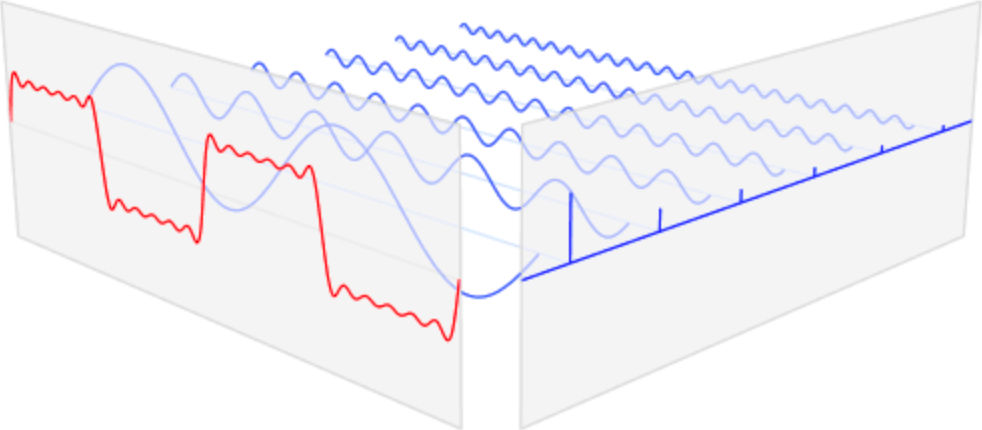
\includegraphics[width=0.6\textwidth]{img/fourier-dimensions.png}
  \caption{Frequency and time domains of a signal. (Image source wikipedia)}
  \label{fig:fourier}
\end{figure}
The wave function in red is the sum of the six waves shown in blue.
The Fourier Transform reveals the amplitudes of the summed sine waves.
Each bar on right side of the image shows a different frequency.  

\section{Practical Example: Denoising Audio Signals}
Let us put aside for the time being the difficulty of the Fourier Transform equations.
Let us pretend that we fully get the meaning of the mathematical equations and apply the Fourier Transform to carry out some useful work in Python~\cite{CleanUpNoise}.

We create two audio signals of different frequencies with the help of Python.
Plots of the individual signals are shown in Figures~\ref{fig:sixty} and \ref{fig:onefifty}.
We then combine them into a single resultant signal through addition.
We call this the clean signal as shown in Figure~\ref{fig:sumsignals}.

Both signals are in the time-domain, as time is on the $x$ axis.
The resultant signal is thus also in the time domain.
\subsection{Generating of two signals and their convolution sum with random noise}
\begin{figure}[H] 
  \centering
  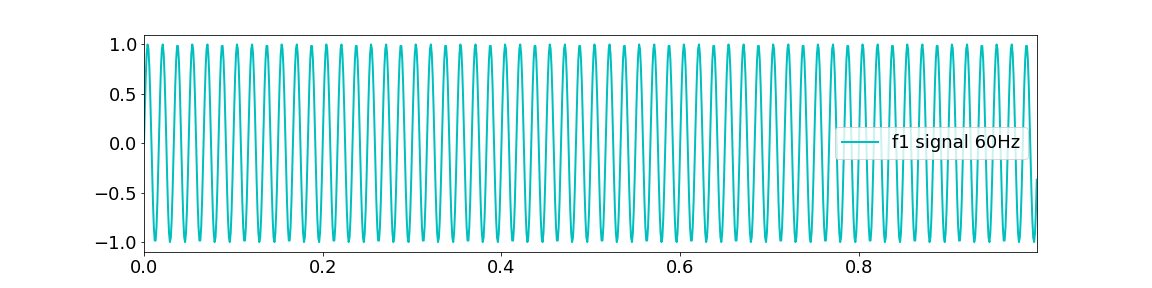
\includegraphics[width=\textwidth]{img/signal_60hz.png}
  \caption{A 60Hz signal.}
  \label{fig:sixty}
\end{figure}

\begin{figure}[H] 
  \centering
  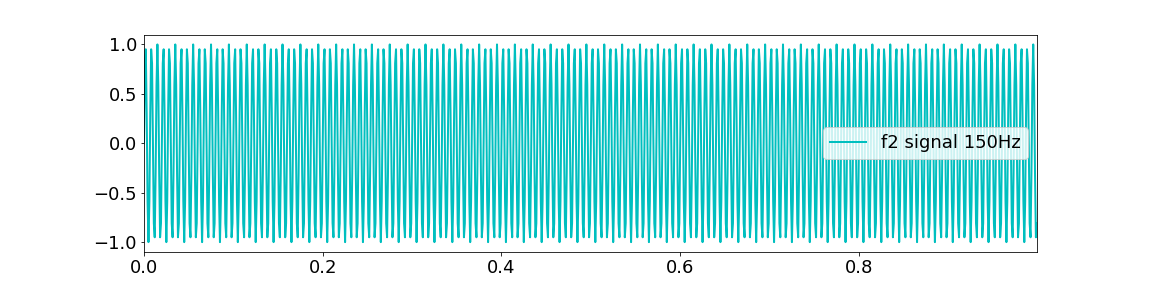
\includegraphics[width=\textwidth]{img/signal_150hz.png}
  \caption{A 150Hz signal.}
  \label{fig:onefifty}
\end{figure}

\begin{figure}[H] 
  \centering
  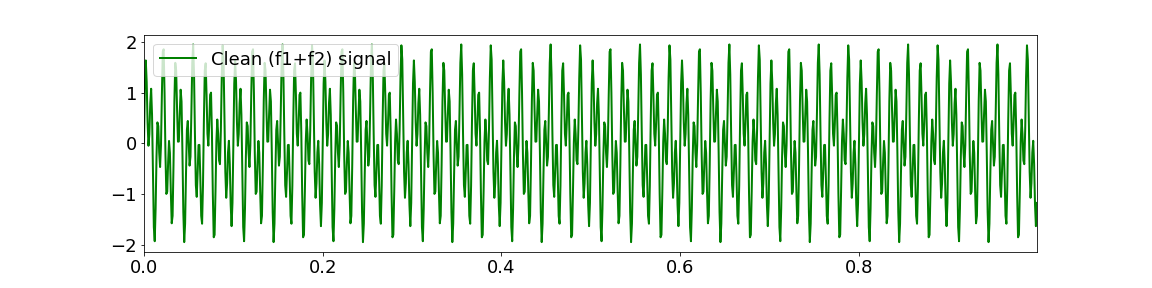
\includegraphics[width=\textwidth]{img/sum_signals.png}
  \caption{Sum of 60Hz and 150Hz signals.}
  \label{fig:sumsignals}
\end{figure}


\subsection{Adding some random noise to original signal}

Next, we deliberately create a random noise signal with random frequency and add it to our clean audio signal.
This is depicted as the red line in Figure~\ref{fig:original_noisy}.
We have superimposed the clean signal in green over it for comparison.
\begin{figure}[H] 
  \centering
  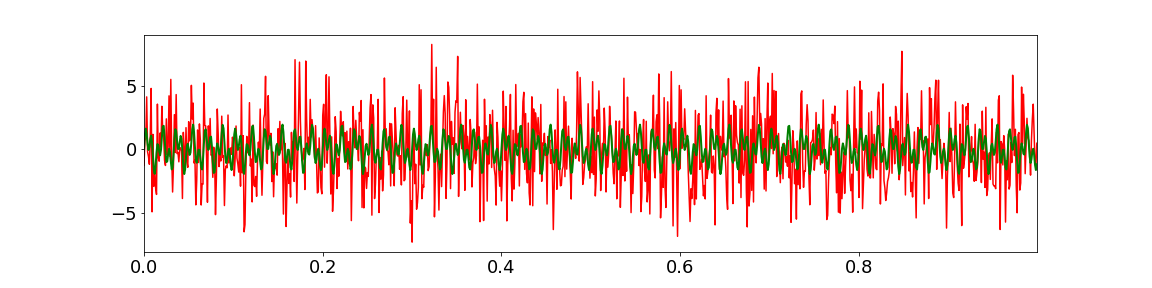
\includegraphics[width=\textwidth]{img/original_noisy.png}
  \caption{The noisy signal with original superimposed.}
  \label{fig:original_noisy}
\end{figure}
Figures~\ref{fig:sixty}, \ref{fig:onefifty}, and \ref{fig:original_noisy} are generated using the Python~\cite{fftnumpy} code in Listing~\ref{listing:sixty}.

\begin{listing}[h]
  \begin{minted}{python}
 #importing libraries and setup
  import numpy as np
  import matplotlib.pyplot as plt
  dt = 0.001 # frame difference 0.001
  t = np.arange(0,1,dt) # time on x-axix
  f1 = np.sin(2*np.pi*60*t) #first signal f1 60Hz
  f2 = np.sin(2*np.pi*150*t) # second singal f2 150Hz
  f_clean= f1 + f2 # suming f1 and f2
  #add some random noise to the signal.
  f = f_clean + 2.5*np.random.randn(len(t))
  \end{minted}
  \caption{Code for time domain signals.}
  \label{listing:sixty}
  \end{listing}
  
\subsection{Converting time domain signal to frequency domain}
We then use Python's numpy library to calculate the DFT of the noisy signal using a FFT.
Figure~\ref{fig:time_to_freq} shows the frequency-domain representation of Figure~\ref{fig:original_noisy}.
It depicts the noisy audio signal that needs to be filtered of noise.
\begin{figure}[H] 
  \centering
  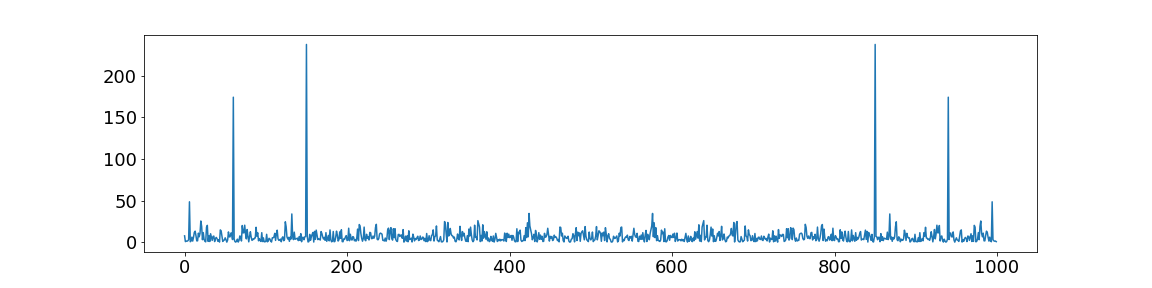
\includegraphics[width=\textwidth]{img/time_to_freq.png}
  \caption{The Frequency domain of the noisy signal.}
  \label{fig:time_to_freq}
\end{figure}
The time domain signal is changed into frequency domain using algorithm we already discussed: an FFT algorithm using the code in Listing~\ref{listing:time_to_freq}.
With the help of the Fourier Transform it becomes easier to track frequencies and break the signal into different frequencies.
The FFT algorithm is the efficient way to do that job.
\begin{listing}[h]
\begin{minted}{python}
# Compute the Fast Fourier Transform (FFT)
n = len(t)
fhat = np.fft.fft(f,n)                     # Compute the FFT
PSD = fhat * np.conj(fhat) / n             # Power spectrum density (power per freq)
freq = (1/(dt*n)) * np.arange(n)           # Create x-axis of frequencies in Hz
L = np.arange(1,np.floor(n/2),dtype='int') # Only plot the first half of freqs
\end{minted}
\caption{Converting time domain to frequency domain with FFT algorithm.}
\label{listing:time_to_freq}
\end{listing}

\subsection{Removing Noise by applying threshold}

In the frequency domain signal, each spike represents a different frequency within the signal.
It is easier to apply threshold to get rid of undesired signals~\cite{fftfilter}.  

If we pick the frequencies that cross the index of 120 in y-axis, we can omit 99\% of the noise because the noise indices are very low.
After applying the threshold of 120 we get the following signal which is totally free from noise, as shown in the Figure~\ref{fig:denoise_freq}.
\begin{figure}[H] 
  \centering
  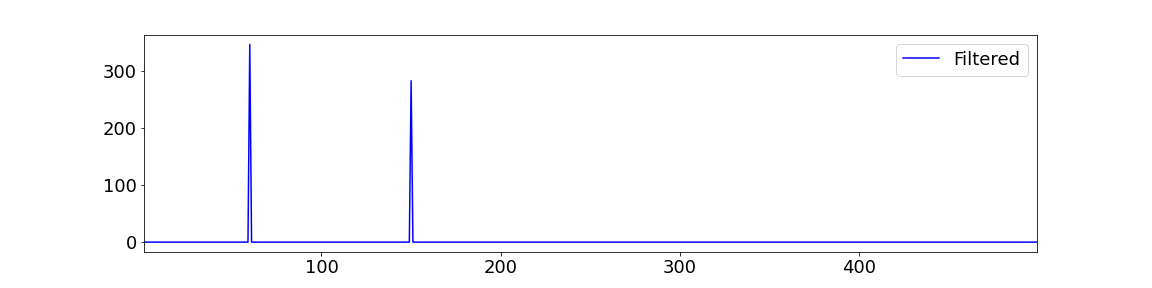
\includegraphics[width=\textwidth]{img/denoise_freq.png}
  \caption{The Frequency domain of the denoised signal.}
  \label{fig:denoise_freq}
\end{figure}
It is still in frequency domain and can be converted back into time domain by doing inverse function of Fast Fourier Transform (IFFT).
This is demonstrated in Listing~\ref{listing:denoise_freq}.
\begin{listing}[H]
\begin{minted}{python}
# Use the PSD (power spectral density) to filter out noise
indices = PSD > 120       # Find all freqs with large power
PSDclean = PSD * indices  # Zero out all others
fhat = indices * fhat     # Zero out small Fourier coeffs. in Y
ffilt = np.fft.ifft(fhat) # Inverse FFT for filtered time signal
\end{minted}
\caption{Noise removed in frequency domain, threshold PSD above 120}
\label{listing:denoise_freq}
\end{listing}

\subsection{Reverting Frequency Domain Signal to Time Domain}
When we apply the inverse FFT, we get a signal in time domain which is almost identical to original summed signal $f$.
Looking at Figure \ref{fig:fft_infft_signals}, we can see the green signal that is the original sum of two signals above.

The signal in blue is the filtered or recovered signal by removing noise.
If both signals are compared there is not any difference and the information in signal is not lost. 
The filtered signal is almost alike the original signal.
\begin{figure}[H] 
  \centering
  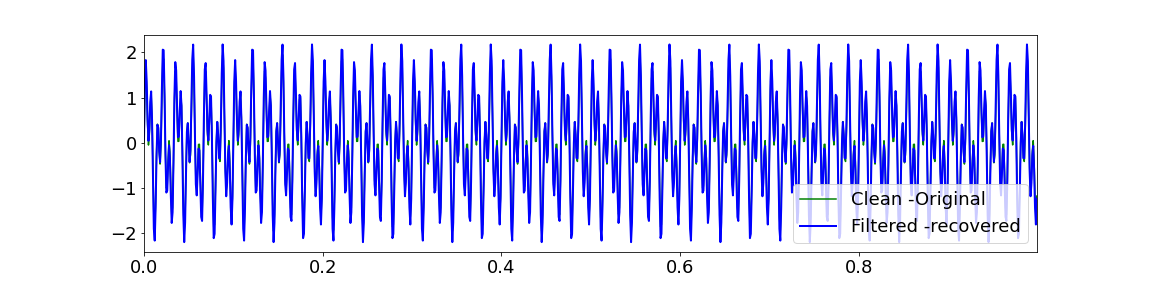
\includegraphics[width=\textwidth]{img/fft_infft_signals.png}
  \caption{Inverse FFT to covert back from frequency to time domain.}
  \label{fig:fft_infft_signals}
\end{figure}

\section{Conclusion}
We provided an overview of Fourier Series, Fourier Transforms and a Fast Fourier Transform (FFT). 
After that, we demonstrated a practical application of the FFT algorithm by denoising the data signal.

Taking advantage of Python, we generated two different signals then added some random noise to it.
We then demonstrated, with help of FFT and inverse FFT, that the noise can be removed from data signals.

The FFT algorithm is the one of the most useful algorithms in common use today~\cite{fftalg}. 
It is used in multiple problem solving approaches such as data cleaning, data analysis, data compression, analog and digital signal processing.

It can also be used for mathematical modelling of PDEs and ODEs systems.
It is also heavily used in quantum mechanics~\cite{QCFFT} and quantum computing~\cite{QFT}.

\newpage
\bibliographystyle{IEEEtran}
\bibliography{bibliography}
\end{document}